\chapter{Methods}

The aim of this thesis is to use inverse design to find a phononic beamsplitter,
a task that can be divided into three parts: 
First, some definitions of what
should be designed and what constitutes a ``good'' design needs to be made.
Second, we need a way to calculate the gradient of the ``goodness'' with respect
to the design.
And lastly, we need a gradient based optimization algorithm to find the optimal
design.
All of this will be described in this chapter.

\todowrt{Comment from PB: at some point you should explain what a beam splitter is, explain why it is so popular in photonics and how it could be interesting in phononics. 
also you should refer to previous work on phononic beam splitters, their plattform and basic differences. 
Doesnt have to be too detailed but some context is required.}

\section{Design}

The device design to be optimized can be seen in \cref{fig:bs-design}.
The input and output waveguides consists of unit cells like the one in
\cref{fig:unitcell}.
The values for the parameters in the sketch are given in \cref{tab:params}.
The reason for using this mode in this waveguide is that it has been shown to be
interesting for avoiding mechanical leakage into the substrate on which it is
clamped, as well as retaining a high optomechanical
coupling.\cite{kolvik_clamped_2023}

Inside the design area, there can be one of two kinds of designs.
The first is a \emph{continuous design}, meaning that the material parameters
$\rho$ and $C_{ijkl}$ are continuously varying. The range of values that they
can take are between the density and elasticity of pure silicon and that of air.
Any in-between values are obviously not something that can be physically
realized, but it is useful as a first step in the optimization.
This is parametrized through the \emph{design field}, $p$, which takes values
between 0, which means pure air, and 1, which means pure silicon.
The second kind is a binary design, where each point either has silicon or not
and there are no in-between values.
This is accomplished using level-set methods, which will be explained in
\cref{sec:level-set}.

Because the device is completely symmetric, only one half of it needs to be
modeled, and the other half is extrapolated with a symmetry boundary condition.

\begin{figure}[htpb]
	\centering
	\def \a{0.5}
\def \w{1.0}
\def \hx{0.13}
\def \hy{0.3}

\tikzset{
	unitcell/.pic={
		\draw[pic actions] (-0.5*\a, -0.5*\w) rectangle (0.5*\a, 0.5*\w);
		\draw[fill=white] (0, 0) circle [x radius=\hx, y radius=\hy];
	}
}

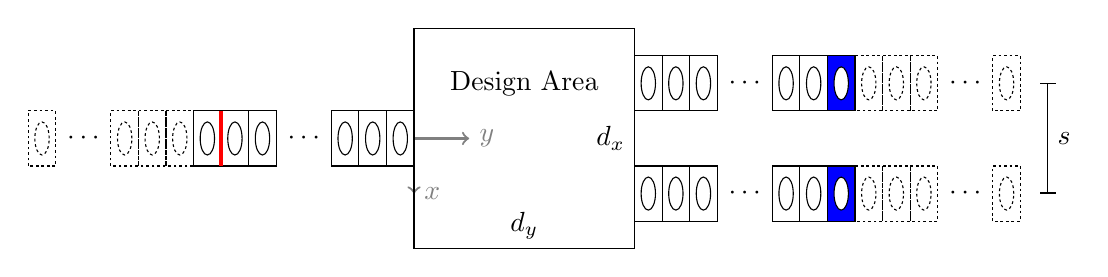
\begin{tikzpicture}[scale=0.7]
	\def \designx{4.0}
	\def \designy{4.0}
	\def \outputh{1.0}
	\def \nunitcells{16}
	\def \nnonpmls{10}

	% Coordinate system
	\draw[gray, thick, ->] (0,0) -- (0,-1) node [anchor=west] {$x$};
	\draw[gray, thick, ->] (0,0) -- (1,0) node [anchor=west] {$y$};

	% Input waveguide
	\path
		(-0.5*\a, 0) pic[transform shape] {unitcell}
		(-1.5*\a, 0) pic[transform shape] {unitcell}
		(-2.5*\a, 0) pic[transform shape] {unitcell}
		(-4.0*\a, 0) node {$\cdots$}
		(-5.5*\a, 0) pic[transform shape] {unitcell}
		(-6.5*\a, 0) pic[transform shape] {unitcell}
		(-7.5*\a, 0) pic[transform shape] {unitcell};
	\draw[red, ultra thick]
		(-7*\a, -0.5*\w) --
		(-7*\a, +0.5*\w);
	\begin{scope}[dash=on 1pt off 1pt phase 0pt]
	\path
		(-8.5*\a, 0) pic[transform shape] {unitcell}
		(-9.5*\a, 0) pic[transform shape] {unitcell}
		(-10.5*\a, 0) pic[transform shape] {unitcell}
		(-12.0*\a, 0) node {$\cdots$}
		(-13.5*\a, 0) pic[transform shape] {unitcell};
	\end{scope}

	% Design area
	\draw (0, -\designx / 2) rectangle (\designy, \designx / 2);
	\node at (\designy / 2, 1) {Design Area};
	\node[left] at (\designy, 0) {$d_x$};
	\node[above] at (\designy/2, -\designx/2) {$d_y$};

	% Output waveguide
	\begin{scope}[xshift=\designy cm, yshift=\outputh cm]
	\path
		(0.5*\a, 0) pic[transform shape] {unitcell}
		(1.5*\a, 0) pic[transform shape] {unitcell}
		(2.5*\a, 0) pic[transform shape] {unitcell}
		(4.0*\a, 0) node {$\cdots$}
		(5.5*\a, 0) pic[transform shape] {unitcell}
		(6.5*\a, 0) pic[transform shape] {unitcell}
		(7.5*\a, 0) pic[transform shape, fill=blue] {unitcell};
	\begin{scope}[dash=on 1pt off 1pt phase 0pt]
	\path
		(8.5*\a, 0) pic[transform shape] {unitcell}
		(9.5*\a, 0) pic[transform shape] {unitcell}
		(10.5*\a, 0) pic[transform shape] {unitcell}
		(12.0*\a, 0) node {$\cdots$}
		(13.5*\a, 0) pic[transform shape] {unitcell};
	\end{scope}
	\end{scope}
	\begin{scope}[xshift=\designy cm, yshift=-\outputh cm]
	\path
		(0.5*\a, 0) pic[transform shape] {unitcell}
		(1.5*\a, 0) pic[transform shape] {unitcell}
		(2.5*\a, 0) pic[transform shape] {unitcell}
		(4.0*\a, 0) node {$\cdots$}
		(5.5*\a, 0) pic[transform shape] {unitcell}
		(6.5*\a, 0) pic[transform shape] {unitcell}
		(7.5*\a, 0) pic[transform shape, fill=blue] {unitcell};
	\begin{scope}[dash=on 1pt off 1pt phase 0pt]
	\path
		(8.5*\a, 0) pic[transform shape] {unitcell}
		(9.5*\a, 0) pic[transform shape] {unitcell}
		(10.5*\a, 0) pic[transform shape] {unitcell}
		(12.0*\a, 0) node {$\cdots$}
		(13.5*\a, 0) pic[transform shape] {unitcell};
	\end{scope}
	\end{scope}
	\draw[|-|]
		(15*\a + \designy, -\outputh) -- node[right] {$s$}
		(15*\a + \designy, \outputh);
		
\end{tikzpicture}

	\caption{
		Device design to be optimized.
		At the red line, a wave traveling right is excited.
		The output is measured over the blue unit cells.
		The dashed unit cells are \glspl{pml}.
		The large, rectangular design area has dimensions $d_x \times d_y \times
		h$.
	}
	\label{fig:bs-design}
\end{figure}
\tododec{Are the dx and dy in \cref{fig:bs-design} clear? I thought of having arrows but it
feels like the image gets quite messy then}

\begin{table}[htpb]
	\centering
	\caption{%
		Values for the geometric parameters of the device.
		Reference \cref{fig:bs-design,fig:unitcell} for what the quantities
		mean.
	}%
	\label{tab:params}

	\begin{tabular}{cc}
		\toprule
		Parameter & value\\
		\midrule
		$a$ & \qty{187}{\nm}\\
		$w$ & \qty{187}{\nm}\\
		$h_x$ & \qty{153.5}{\nm}\\
		$h_y$ & \qty{49.5}{\nm}\\
		$h$ & \qty{220}{\nm}\\
		$d_x$ & $6 w$\\
		$d_y$ & $4 w$\\
		$s$ & $3 w$\\
		\bottomrule
	\end{tabular}
\end{table}

\tododec{Write about why we use the mode we use, and why I clamp the bottom. Can
reference Johan and Pauls paper}

\subsection{Objective function}

The figure of merit of the device is how much of the input excitation gets transmitted
into the output beams.
Furthermore, all of the excitation of the output waveguide should be in the same
mode that was excited at the input.
Therefore, a mode overlap integral is used:
\begin{equation}
	I = \int_{\Omega_1} \vec{m}^*(\vec{x}) \vec{u}(\vec{x}) \dl{\vec x},
\end{equation}
where $\vec m$ is the shape of the mode (\cref{fig:ms1}).
Because we are not interested in the phase of the output waves,
the absolute value squared of the overlap integral is taken as the objective
function,
\begin{equation}
	\fobj = \abs{I}^2 = I I^*.
\end{equation}
This will be maximized when the excitation of the mode $m$ in the output
waveguide is maximized, regardless of which phase it has.

The functional derivative of $\fobj$ with respect to $p$ then becomes
\begin{align}
	\diff.f.{\fobj}{p}(x) &= \diff.f.{I}{p}(x) I^* + I\diff.f.{I^*}{p}(x)\\
	&= \diff.f.{I}{p}(x) I^* + \left(I^*\diff.f.{I}{p}(x)\right)^*\\
	&= 2\Re\left(\diff.f.{I}{p}(x) I^*\right).
\end{align}
The derivative of $I$ was derived in \cref{sec:spec_der}.

\tododec{Paragraph about pure part of objective function, enforcing the minimum
feature size}

\subsection{Excitation}

In order to excite the input waveguide in the desired mode,
the stress on the boundary of a unit cell was exported from a unit cell
eigenmode simulation with $k=0.9 \pi / a$ and applied to the boundary marked in red in
\cref{fig:bs-design}.
Since the frequency is perfectly controlled, this should excite only the desired
mode, since that is the only permitted mode close by as seen in the band diagram
in \cref{fig:banddiagram}.

In order to confirm that the excitation was indeed fully in the desired mode, a
separate model with only a waveguide with 200 unitcells was created.
After applying the excitation and running the simulation,
the proportion of the excitation that ended up in the desired mode was
calculated.
This was done by first calculating the mode overlap integral
$\int u u_m^* \dl{\vec x}$
and comparing that to the norm of the displacement field
$\int u u^* \dl{\vec x}$.
If $u = a u_m + b u_r$ for some scalars $a$ and $b$, then
$\int u u^* \dl{\vec x} = a\int u u_m^*\dl{\vec x} + b\int u u_r^*\dl{\vec x}$.
And assuming $u_r$ is orthogonal to $u_m$,
$a = \int u u_m^*\dl{\vec x} / \int u_m u_m^*\dl{\vec x}$.
% the mode overlap integral
% was then calculated, as well as the integral $\int u_i^* u_i$ from which one can
% calculate the proportion of energy in the mode compared to the energy in other
% modes.
The result was near perfect ($b < 0.01 a$) excitation of only the desired mode.
To obtain such high fidelity, it was important that the mesh used for the
unitcells in the wave guide was the same as the mesh in the unit cell
simulation.
High fidelity was also achieved if both meshes were made very fine, but such
fine meshes carries a prohibitively large computational cost.

\subsection{Perfectly Matched Layers (PMLs)}

\tododec{Humour?}
Ideally, the input and outputs are infinite waveguides.
Unfortunately, it has been discovered that infinity is big; simulating
infinite waveguides would take infinite time, and the author would like to be done by
June.
Instead, \glspl{pml} are placed at the caps of the input and output waveguides.
The purpose of the \gls{pml} is to absorb any incoming waves without reflection,
which would make it act as if there was an infinite waveguide on the other side
into which the waves propagate indefinitely.
The way to accomplish this is to add an imaginary component to the density of
the material.
This needs to be done smoothly, otherwise the abrupt change in material
parameters would induce reflections anyway.
Therefore, the imaginary part is taken to be exponentially increasing.
Furthermore, the curve is shifted vertically such that it is 0 at $y = y_0-n$,
and rescaled so that it is $\rho_\text{si} s$ at $y=y_0$.
\begin{equation}
	\rho_\text{im} = \rho_\text{si} \cdot s \cdot
	\frac{e^{-\abs{y-y_0} / d} - e^{-n/d}}{1 - e^{-n/d}}
\end{equation}
\Cref{fig:pml_profile} shows the effect of changing these parameters on the
shape of the profile of the imaginary component.

\todowrt{Explain why adding an imag part absorbs waves}

\begin{figure}[htpb]
	\centering
	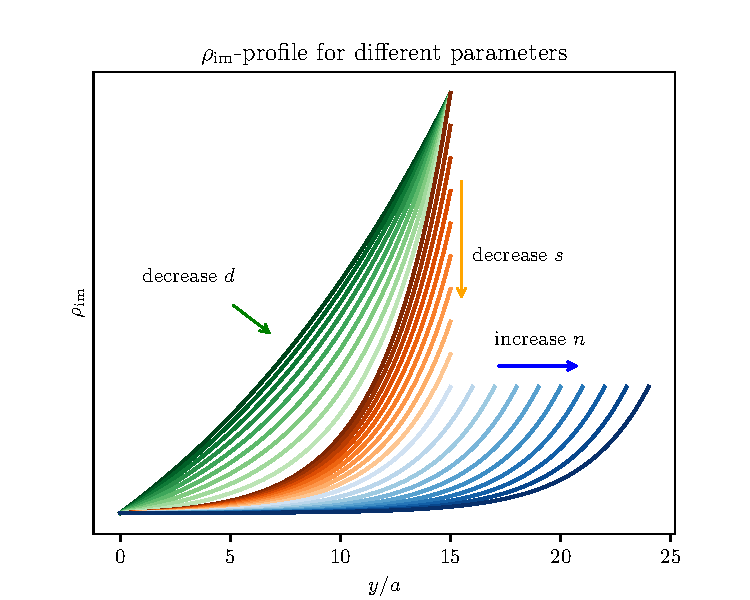
\includegraphics{chapters/methods/pml_profile.pdf}
	\caption{
		This figure shows the effect of changing different parameters.
		The green curves shows changing $d$ while keeping the other parameters
		fixed, and the orange and blue show $s$ and $n$ respectively.
		Darker colour means higher value, and the last green curve coincides
		with the first orange, and the last orange with the first blue.
	}
	\label{fig:pml_profile}
\end{figure}

There are three possible sources of reflections.
Firstly, if the transition from no imaginary component to some imaginary
component is too abrupt, that causes reflections.
Secondly, if the imaginary component is too small, the waves will not be
dampened completely when they reach the end of the \gls{pml} and thus reflect
off of that.
And lastly, if $d$ is small then there can be reflections from the steep
increase that happens some distance away from the beginning of the \gls{pml}.
See \cref{fig:banddiagram} for an illustration of where the different types of
reflections occur.

\tikzset{
	reflection/.pic={
		\draw[->] (-0.4, 0) -- (-0.1, 0) arc[radius=0.1, start angle=-90, end
		angle=90] --++ (-0.1, 0);
		\draw[dashed] (0,-3.1) -- (0,8.3);
	}
}
\begin{figure}[htpb]
	\centering
	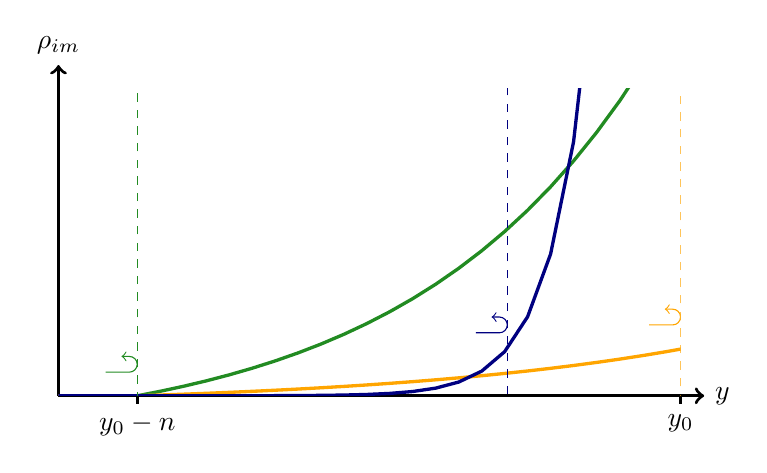
\begin{tikzpicture}[domain=1:8]

		\draw[->,very thick] (-0.0,0) -- (8.2,0) node[right] {$y$};
		\draw[->,very thick] (0,-0.0) -- (0,4.2) node[above] {$\rho_\text{im}$};
		\draw[very thick] (1,0) -- (1,-0.10) node[below] {$y_0-n$};
		\draw[very thick] (7.9,0) -- (7.9,-0.10) node[below] {$y_0$};
		%\draw[very thin,color=gray] (-0.1,-1.1) grid (7.9,3.9);
		\clip (0.0, 0.0) rectangle (7.9,3.9);
		\draw[color=ForestGreen, very thick] (0,0) -- (1,0) --
			plot (\x,{0.40*(exp(\x/3)-exp(1/3))});
		\draw[color=Orange, very thick] (0,0) -- (1,0) --
			plot (\x,{0.10*(exp(\x/4)-exp(1/4))});
		\draw[color=NavyBlue, very thick] (0,0) -- (1,0) --
			plot (\x,{0.02*exp(2.0*(\x-4))});
		\draw[ForestGreen] (1.0, 0.3) pic {reflection};
		\draw[NavyBlue] (5.7, 0.8) pic {reflection};
		\draw[Orange] (7.9, 0.9) pic {reflection};
	\end{tikzpicture}
	\caption{
		For the green curve, the initial sudden increase of the imaginary
		component of the density at the beginning of the \gls{pml} causes reflections.
		For the blue curve, the beginning of the \gls{pml} is smooth but there
		is an increase partway through sharp enough to cause reflections.
		For the orange curve, the \gls{pml} never becomes strong enough to
		completely dampen the waves, and they get reflected at the end.
	}
	\label{fig:pml_reflections}
\end{figure}

It is desirable to make $n$ as small as possible while still eliminating all
reflections. In order to do so, a long waveguide with the same parameters as
used for the input and output waveguides in the beamsplitter design was created.
To discern where there was some component of the wave reflected, a fourier
transform of the displacement field was made.
\Cref{fig:pml_sweep1} shows the amplitude of the reflection,
quantified as the peak height relative to the forward propagating wave,
for different profiles.
These figures fit well with the three types of reflection mentioned previously.
To achieve a short yet functional \gls{pml}, $d=5$, $s=0.03$ and $n=20$ was
chosen.

\begin{figure}[htpb]
	\centering
	\begin{subfigure}[]{\textwidth}
	\begin{center}
		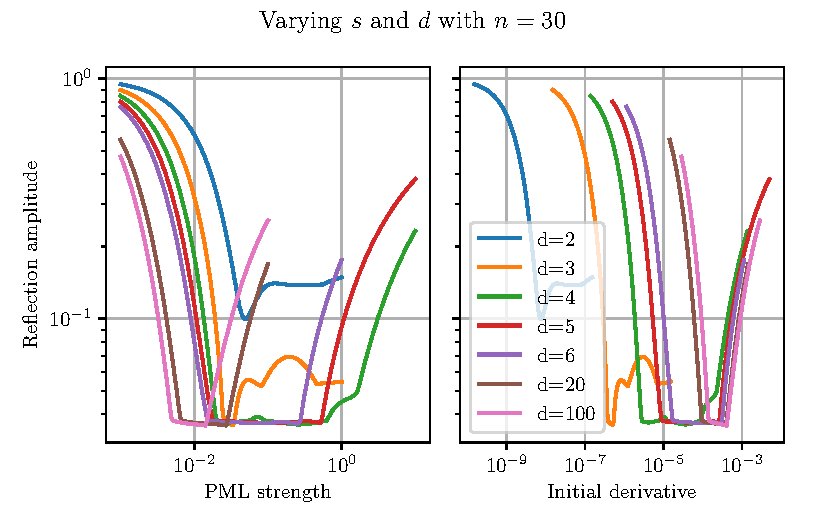
\includegraphics{chapters/methods/pml_sweep_sd.pdf}
	\end{center}
	\caption{
		On the left is the reflection amplitude plotted as a function of the
		\gls{pml} strength $s$ for different $d$.
		For $d > 4$ there are two sources of reflection:
		for small $s$ reflection at the end of the \gls{pml} occurs,
		and for large $s$, there is reflection at the beginning.
		The right figure makes it clear that it is the slope at the beginning of
		the \gls{pml} that matters, since the point at which it becomes
		significant is the same for all $d$.
	}
	\label{fig:pml_sweep_sd}
	\end{subfigure}
	\begin{subfigure}[]{\textwidth}
	\begin{center}
		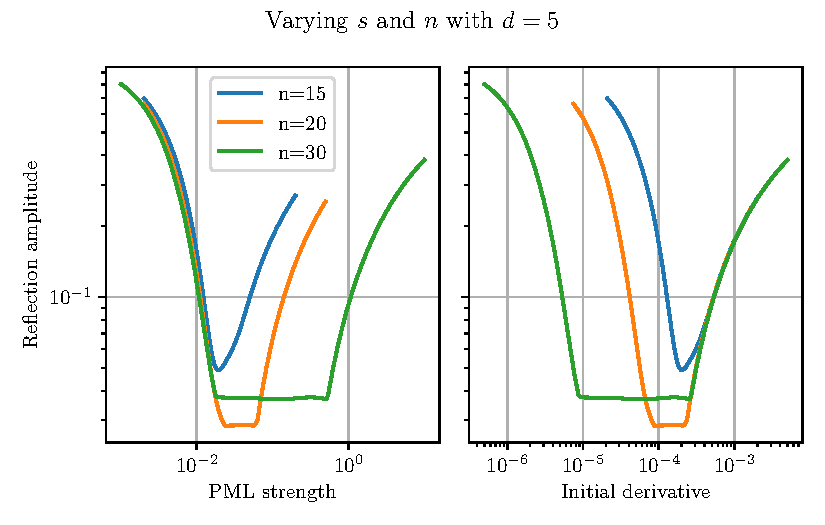
\includegraphics{chapters/methods/pml_sweep_sn.pdf}
	\end{center}
	\caption{
		This is the same as \cref{fig:pml_sweep_sd} but with varying $n$.
		For $n=15$, the reflections from the beginning do not subside before the
		reflections from the end become significant, so at least $n=20$ is
		necessary.
	}
	\label{fig:pml_sweep_sn}
	\end{subfigure}
	\caption{}
	\label{fig:pml_sweep1}
\end{figure}

\subsection{Level-set}\label{sec:level-set}

Ultimately, we want our device to consist of regions of material and regions of
no material.
There are basically two ways of doing this.
The first, and perhaps most intuitive,
is to simply store the coordinates of the boundary between the filled and empty
regions.
In addition to storing the coordinates, one must also store which points
neighbour which.
The second method, which is the one used in this report, is called
the \emph{level-set method}.
In this method, the boundary is not directly stored, but rather is stored via an
\emph{implicit function}, $\phi(x)$, defined such that the boundary is the
0-isocontour of $\phi$, i.e.\ the points $x$ where $\phi(x)=0$.

There are two main advantages of using the level-set method rather than
directly storing the boundary points.
Firstly, when moving the boundary we would like to do so in the normal
direction, as moving it along itself has no effect.
Computing the normal direction of a directly stored boundary is slightly cumbersome,
though certainly achievable.
With level-set, moving the boundary in the normal direction is as easy as adding
a constant to the implicit function.
Secondly, while the boundary is changing, the resolution in one part might need
to be increased while the resolution in another needs to be decreased. Deciding
where and when to add new points is non-trivial when directly storing the
boundary. Furthermore, if two boundaries merge, or if one splits in two, points
need to be removed and the connectivities changed, which is quite complex.
\Cref{fig:direct_troubles} illustrates these problems with direct storage concretely.
Both of these issues are automatically handled with the level-set method.
\tododec{How? (Isn't it obvious?)}

\begin{figure}[htpb]
	\centering
	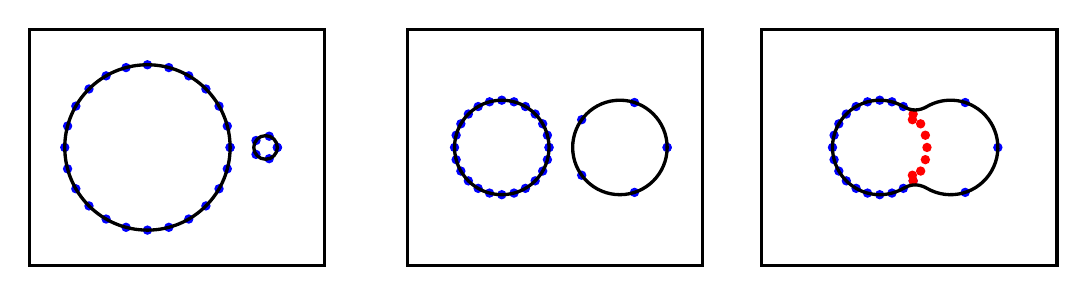
\begin{tikzpicture}[scale=1.5, very thick]
	\coordinate (ca) at (0,0);
	\coordinate (cb) at (1,0);
	\def\radiusa{0.7cm}
	\def\radiusb{0.1cm}
	\def\radpt{0.7pt}
	\draw (-1,-1) rectangle (1.5,1);
	\foreach \i in {0,15,...,360}{% 
		\filldraw [blue]  (ca)++(\i:\radiusa) circle (\radpt);
	}
	\foreach \i in {0,72,...,360}{% 
		\filldraw [blue]  (cb)++(\i:\radiusb) circle (\radpt);
	}
	\draw (ca) circle[radius=\radiusa];
	\draw (cb) circle[radius=\radiusb];

	\begin{scope}[xshift=3cm]
		\coordinate (ca) at (0,0);
		\coordinate (cb) at (1,0);
		\def\radiusa{0.4cm}
		\def\radiusb{0.4cm}
		\draw (-0.8,-1) rectangle (1.7,1);
		\foreach \i in {0,15,...,360}{% 
			\filldraw [blue]  (ca)++(\i:\radiusa) circle (\radpt);
		}
		\foreach \i in {0,72,...,360}{% 
			\filldraw [blue]  (cb)++(\i:\radiusb) circle (\radpt);
		}
		\draw (ca) circle[radius=\radiusa];
		\draw (cb) circle[radius=\radiusb];
	\end{scope}
	\begin{scope}[xshift=6cm]
		\coordinate (ca) at (0.2,0);
		\coordinate (cb) at (0.8,0);
		\def\radiusa{0.4cm}
		\def\radiusb{0.4cm}
		\draw (-0.8,-1) rectangle (1.7,1);
		\foreach \i in {60,75,...,315}{% 
			\filldraw [blue]  (ca)++(\i:\radiusa) circle (\radpt);
		}
		\foreach \i in {-72,0,72}{% 
			\filldraw [blue]  (cb)++(\i:\radiusb) circle (\radpt);
		}
		\foreach \i in {-45, -30, ..., 45}{% 
			\filldraw [red]  (ca)++(\i:\radiusa) circle (\radpt);
		}
		\foreach \i in {144, -144}{% 
			\filldraw [red]  (cb)++(\i:\radiusb) circle (\radpt);
		}
		\draw (ca)++(60:\radiusa)
			arc[radius=\radiusa, start angle=60, end angle=300]
			to[out=30, in=150]
			([shift=(240:\radiusb)] cb)
			arc[radius=\radiusb, start angle=240, end angle=480]
			to[out=210, in=-30]
			cycle;
		%\draw (cb) circle[radius=\radiusb];
	\end{scope}
\end{tikzpicture}

	\caption{%
		Possible evolution of boundary. In the leftmost figure, the
		boundary is defined by pretty much evenly spaced points. In the center figure
		the boundaries have moved and the spacing is no longer even, and the
		right circle is very poorly resolved.
		The rightmost figure shows the boundary after the two circles moved
		closer together. Now there are multiple points that need to be removed,
		marked in red, and the connectivity of the points that remain must be
		changed such that the two boundaries are merged.
	}
	\label{fig:direct_troubles}
\end{figure}
\begin{figure}[htpb]
	\centering
	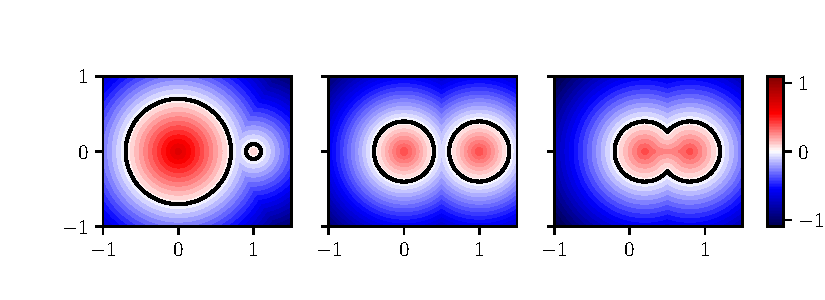
\includegraphics{chapters/methods/signed_dist_example.pdf}
	\caption{%
		Example of three signed distance functions for three different
		boundaries.
	}
	\label{fig:signed_dist_example}
\end{figure}

There are of course a lot of possible functions $\phi(x)$ that have a given
boundary as it's 0-isocontour.
There is one choice that simplifies a lot of calculations though: the signed
distance function.
This function is defined as the distance from the closest point on the boundary,
with a plus sign if it is inside and a minus sign if it is outside the boundary.
See \cref{fig:signed_dist_example} for an example.
It has the advantage that if one wishes to locally shift the boundary some
length $s$ in the normal direction, then simply add $s$ to the function there.
\Cref{fig:add_shift} shows this effect in one dimension.
\todowrt{
	Create another figure that shows it in two dimensions.
	I'm thinking a circular boundary, and adding $s$ in the left half and
	subtracting $s$ in the right half. Alternatively adding $s\cdot x$ (unit circle
	centered on 0) so that it will be smooth
}

\begin{figure}[htpb]
	\centering
	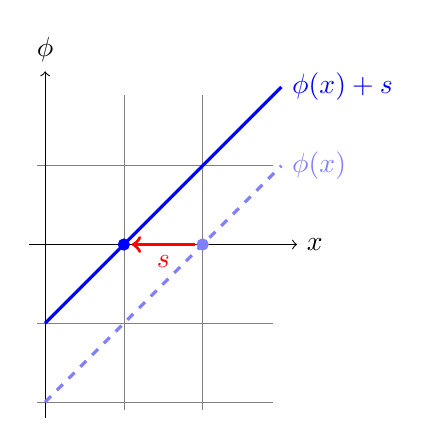
\begin{tikzpicture}[domain=0:3]
		\draw[very thin,color=gray] (-0.1,-2.1) grid (2.9,1.9);

		\draw[->] (-0.2,0) -- (3.2,0) node[right] {$x$};
		\draw[->] (0,-2.2) -- (0,2.2) node[above] {$\phi$};
		\draw[color=blue!50, dashed, very thick] plot (\x,{\x-2})
			node[right] {$\phi(x)$};
		\draw[color=blue, very thick] plot (\x,{\x-1})
			node[right] {$\phi(x)+s$};
		\filldraw[color=blue!50] (2,0) circle[radius=2pt];
		\filldraw[color=blue]    (1,0) circle[radius=2pt];
		\draw[color=red, ->, very thick] (1.9,0) --
			node[below] {$s$}
			(1.1,0);
	\end{tikzpicture}
	\caption{Adding $s$ to the signed distance function shifts boundary by $s$.}
	\label{fig:add_shift}
\end{figure}

Using a signed distance function means that a gradient descent step can be taken
by simply adding the gradient field to the signed distance field.
However, there are some pitfalls that must be avoided.
Firstly, the gradient needs to be rescaled so that the boundary moves
an appropriate distance.
This has been done such that the boundary moves maximally \qty{5}{\nm}.
\todoblk[noinline]{check this number before finalizing, I change it every now and then}
Secondly, since the gradient is occasionally sharply peaked somewhere which may
not lie near the boundary, only the gradient near the boundary is actually added
to the signed distance field.
After performing this addition, what was previously a signed distance field will
now no longer be that, and thus the signed distance field is recalculated from
the new boundary.
This recalculation comes with a performance penalty, but since the COMSOL
simulations are orders of magnitude slower than all other parts of the
optimization, this is of little concern.

\tododec{Meshing of the level-set designs?}

\section{Simulations}

\tododec{
	How much specifics should I have? Should I write about exporting the
	gradient to a file and how I calculate the 2D gradient in my matlab scripts
	from that
}
\todowrt{Mesh export / import and why that is done should probably be mentioned
since it's quite important to get the excitation in the right mode.}

\section{Optimization}

\tododec{%
	Describe what optimization algorithm was used, as well as how this
	changed during the simulation. E.g.\ first 200 iterations ADAM; next ADAM
	but with sigmoid function application; sigmoid + feature size; and finally level-set.
}
